\section*{Background}
\addcontentsline{toc}{section}{\protect\numberline{}{Background}}

% intuitive problem statements
\paragraph{Problems} In this thesis we consider the problem of pairwise sequence
alignment: given two sequences, one has to be aligned to the other in a way that
minimizes the aligning differences. More specifically, we minimize the number of
substitutions, insertions and deletions of single letters that have to be
applied to one of the sequences in order to perfectly align to the other. As
shown on~\cref{fig:alignment-types}, there are multiple alignment types but in
this thesis we limit our attention to global and semi-global alignment only. If
both sequences have to be aligned end to end, we call it a \emph{global
alignment} and the number of differences is \emph{edit distance}. If instead we
search for an alignment of the first sequence somewhere within the second (so we
are free to skip the beginning and the end of the second sequence), such an
alignment is called \emph{semi-global}. 

%\begin{floatingfigure}[l]{0.5\textwidth}
\begin{figure}[t]
    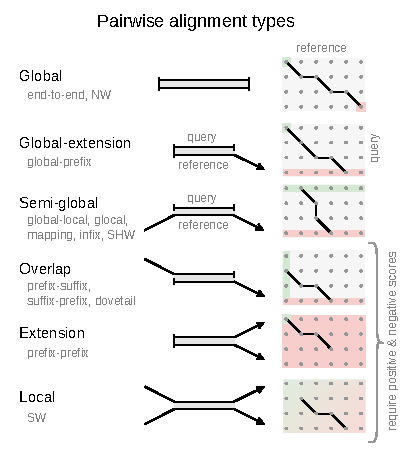
\includegraphics[width=0.5\textwidth]{alignment-types}
	\caption[Alignment types]{Alignment types.}
    \label{fig:alignment-types}
\end{figure}

\paragraph{Applications} Commonly in bioinformatics, the high-throughput
sequencing data consist of a great number of genomic sequences that have to be 

% first effiecient solutions
\paragraph{First solutions} The global alignment problem has been efficiently
solved for a first time around
\citeyear{vintsyuk1968speech}~\cite{vintsyuk1968speech,needleman1970general}.
The problem of approximate/fuzzy string search (semi-global alignment of one
query) has been efficiently approached a decade later, in
\citeyear{sellers1980theory}~\cite{sellers1980theory,smith1981identification}.
more recent and additionally to the issues with handling errors, a new dimension
of complexity appears by the need to locate the position in the reference. The
problem of searching for multiple sequencing has been approached
since\citeyear{pearson1988improved}~\cite{pearson1988improved} and became
central to read alignment of high-throughput sequencing. The specifics with
semi-global alignment requires a trie-like index which is well-used in the
fiels, and known since
\citeyear{thue1912gegenseitige}~\cite{thue1912gegenseitige} and used in
informatics since~\citeyear{de1959file}~\cite{de1959file}.

An important factor for the development of the sequencing algorithms is the
technological advancement~\cite{alser2021technology}. One possible reason is the
combination of massive new data and advancement in computation hardware allowing
for various kinds of parallelization.
%Thus the advancements with bit-parallel algorithms (CITE Myears, Mikko).

% parallelization
% sketches

% Optimal DP-based approaches
\paragraph{Optimal alignment}
Current optimal alignment algorithms reach the impractical $\Oh(nm)$ runtime
that has been shown to be a lower bound for the worst-case edit distance
computation~\cite{backurs2015edit}. In this light, approaches for improving the
efficiency of optimal alignment have taken advantage of specialized features of
modern CPUs to improve the practical runtime of the Smith-Waterman dynamic
programming (DP) algorithm~\cite{smith_comparison_1981} considering all possible
starting nodes. These use modern SIMD instructions (\eg
\vg~\cite{garrison_variation_2018} and \pasgal~\cite{jain_accelerating_2019}) or
reformulations of edit distance computation to allow for bit-parallel
computations in \graphaligner \footnote{We refer as \bitparallel to to the
bit-parallel DP algorithm implemented in \graphaligner tool
\cite{rautiainen_bitparallel_2019}.}~\cite{rautiainen_bitparallel_2019}. Many of
these, however, are designed only for specific types of genome graphs, such as
{\itshape de Bruijn}
graphs~\cite{liu_debga_2016,limasset2019toward} and
variation graphs~\cite{garrison_variation_2018}. A compromise often made when
aligning sequences to cyclic graphs using algorithms reliant on directed acyclic
graphs involves the computationally expensive ``DAG-ification'' of graph
regions~\cite{kavya_sequence_2019,garrison_variation_2018}.

\paragraph{Seed-and-Extend}
Since optimal alignment is often intractable, many aligners use heuristics, most
commonly the \emph{seed-and-extend}
paradigm~\cite{altschul_basic_1990,langmead_fast_2012,li_fast_2009}. In this
approach, alignment initiation sites (\emph{seeds}) are determined, which are
then \emph{extended} to form the \emph{alignments} of the query sequence. The
fundamental issue with this approach, however, is that the seeding and extension
phases are mostly decoupled during alignment. Thus, an algorithm with a provably
optimal extension phase may not result in optimal alignments due to the
selection of a suboptimal seed in the first phase. In cases of high sequence
variability, the seeding phase may even fail to find an appropriate seed from
which to extend.

\paragraph{Known limitations}

Quadratic optimal for semi-global